\renewcommand{\thechapter}{\Alph{chapter}}
\setcounter{chapter}{0}

\titleformat{\chapter}[display]
	{\large\centering}{[{\appendixname\ \thechapter}]}{0pt}{\large}
	\titlespacing{\chapter}
	{0pt}{-20pt}{30pt}
	
% \titlecontents{chapter}% <section-type>
%     [3.22cm]% <left>
%     {\addvspace{0pt}}% <above-code>
%     {\hspace{-3.22cm}\MakeUppercase{\bfseries\appendixname}\hspace{0.1em}
%     \makebox[10pt][l]{\bfseries\thecontentslabel}\bfseries\quad\uppercase}% <numbered-entry-format>
%     {}% <numberless-entry-format>
%     {\titlerule*[8pt]{.}\contentspage}[\addvspace{0pt}]


\addtocontents{toc}{\protect\value{tocdepth}=-1}

% --------------------------------------------------------------------
% Anexos -------------------------------------------------------------

\includepdf[scale=0.7,pages=1,pagecommand=\chapter{[Informe académico]}\addtocontents{toc}{\protect\value{tocdepth}=1}
\phantomsection
\addcontentsline{toc}{chapter}{ANEXOS}
\addtocontents{toc}{\protect\value{tocdepth}=-1}]{imagenes/informeAcademico}

\includepdf[scale=0.7,pages=2, pagecommand={}]{imagenes/informeAcademico}

%\chapter{[Otro anexo]}
